\documentclass[
    report,
    11pt,
    oneside,
    a4paper,
    english,
    brazil,
    sumario=tradicional
    ]{abntex2}

% Pacotes fundamentais
\usepackage{lmodern}
\usepackage[T1]{fontenc}
\usepackage[utf8]{inputenc}
\usepackage{indentfirst}
\usepackage{nomencl}
\usepackage{color}
\usepackage{microtype}
\usepackage{graphicx}
\graphicspath{{img/}}

% Pacotes adicionais
\usepackage{lipsum}
% \usepackage[brazilian,hyperpageref]{backref}
\usepackage[alf]{abntex2cite}

% % Configurações do pacote backref
% \renewcommand{\backrefpagesname}{Citado na(s) página(s):~}
% \renewcommand{\backref}{}
% \renewcommand*{\backrefalt}[4]{
%     \ifcase #1
%         Nenhuma citação no texto.
%     \or
%         Citado na página #2.
%     \else
%         Citado #1 vezes nas páginas #2.
%     \fi}%

\title{Viés da Negatividade em Redes Sociais}
% \tituloestrangeiro{\textbf{How the GDPR Failed} \\ \Large{And how we can still succeed}}

\autor{Pedro Sader Azevedo}
\instituicao{Universidade Estadual de Campinas}
\local{Brasil}

% Configurações de aparência do PDF final
% alterando o aspecto da cor azul
\definecolor{blue}{RGB}{41,5,195}

\makeatletter
\hypersetup{
   pagebackref=true,
   pdftitle={\@title},
   pdfauthor={\@author},
   pdfsubject={A complexidade do problema da desigualdade salarial entre homens e mulheres},
   pdfcreator={LaTeX with abnTeX2},
   pdfkeywords={ods}{gênero}{salário}{ocupação},
   colorlinks=true, % false: boxed links; true: colored links
   linkcolor=blue, % color of internal links
   citecolor=blue, % color of links to bibliography
   filecolor=magenta, % color of file links
   urlcolor=blue,
   bookmarksdepth=4
}
\makeatother

% compila o indice
\makeindex

% margens
\setlrmarginsandblock{3cm}{3cm}{*}
\setulmarginsandblock{3cm}{3cm}{*}
\checkandfixthelayout

% tamanho da indentação
\setlength{\parindent}{1.3cm}

% espaçamento entre parágrafos
\setlength{\parskip}{0.2cm}
% \setlength{\onelineskip}

\SingleSpacing


\begin{document}

\selectlanguage{brazil}

\frenchspacing

\maketitle

\pagenumbering{gobble}

\textual

    O viés da negatividade é a tendência a reagir mais intensamente a informações negativas que positivas~\cite{bad-stronger-than-good}. No contexo das redes sociais, esse viés dificulta a comunicação não-violenta e favorece a disseminação de discursos odiosos e informações falsas.

    Isso ocorre, pois as redes sociais potencializam os efeitos do viés da negatividade por meio de dois mecanismos. O primeiro deles é o algoritmo que promove postagens de acordo com métricas de engajamento, frequentemente priorizando aquelas que despertam emoções negativas~\cite{negativity-spreads-wide, negativity-virality}. O segundo, é o aumento massivo da suscetibilidade ao contágio emocional. Exemplo disso, é que usuários mais expostos a conteúdos negativos fazem mais postagens da mesma natureza~\cite{massive-emotional-contagion}, em um sistema de retroalimentação.

\begin{figure}[htb]
    \caption{\label{charge}``Redes Sociais''}
    \centering
    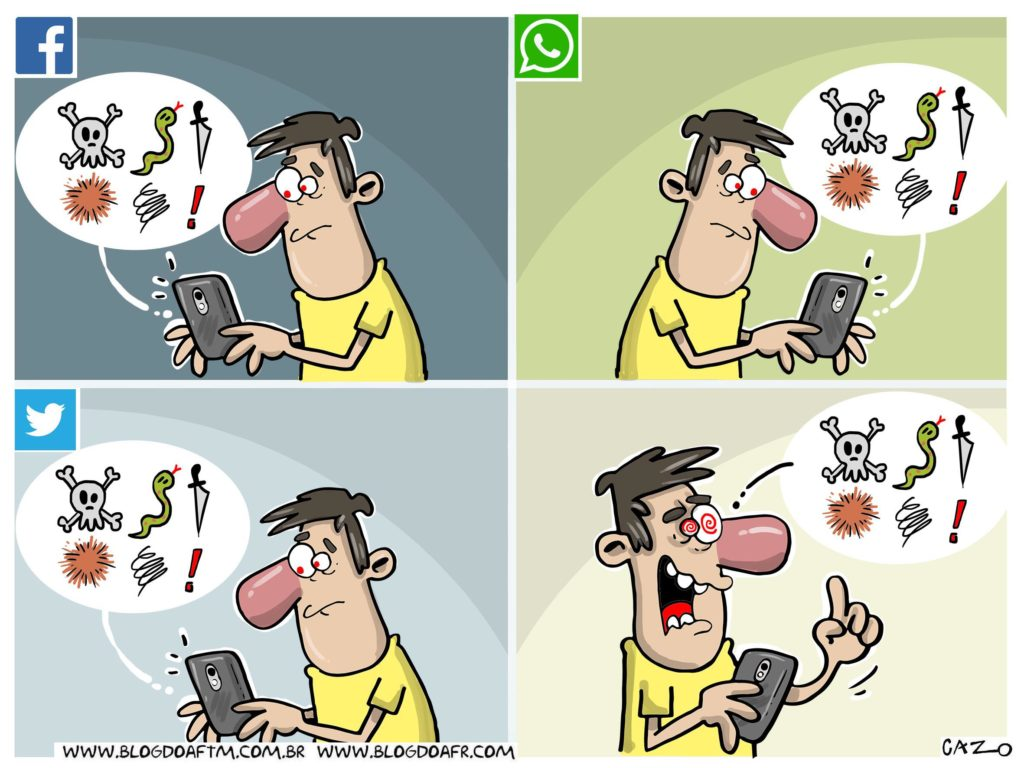
\includegraphics[width=0.8\textwidth]{charge.jpg}
    \fonte{Blog do AFTM\protect\footnotemark}
\end{figure}
\footnotetext{Disponível em \url{https://blogdoaftm.com.br/charge-redes-sociais/}. Acesso em: 7 jun. 2021}

    O problema disso é que ficamos cada vez mais expostos a pontos-de-vista inegavelmente danosos a nossas interações sociais. De acordo com o Relatório Anual do OHCHR (\textit{Office of the High Commissioner for Human Rights}) as ocorrências de discurso de ódio contra minorias dispararam em 2020, em especial contra mulheres e negros~\cite{hate-speech-increasing}. Não por coincidência, são também esses grupos que mais sofrem com os negacionismos difundidos em redes sociais. No caso do negacionismo histórico, desprezam a importância da matriz africana para a formação cultural e econômica do Brasil, contribuindo para o aprofundamento do preconceito e da desigualdade racial. No caso do negacionismo científico, minimizam a responsabilidade humana pelas mudanças climáticas, levando a intensificação de desastres ``naturais'' que afetam a demografia feminina de forma desproporcionalmente severa~\cite{clima-mulheres}.

% Incluir entradas não citadas no texto na bibligrafia
\nocite{manipulation-for-science, be-mean-online}

\pagebreak

\postextual

\bibliography{ref}

\end{document}
